
\section{Experiments}


%
% Simple topology
%
\begin{frame}\frametitle{Simple topology}

	\begin{figure}[h]
        \centering
        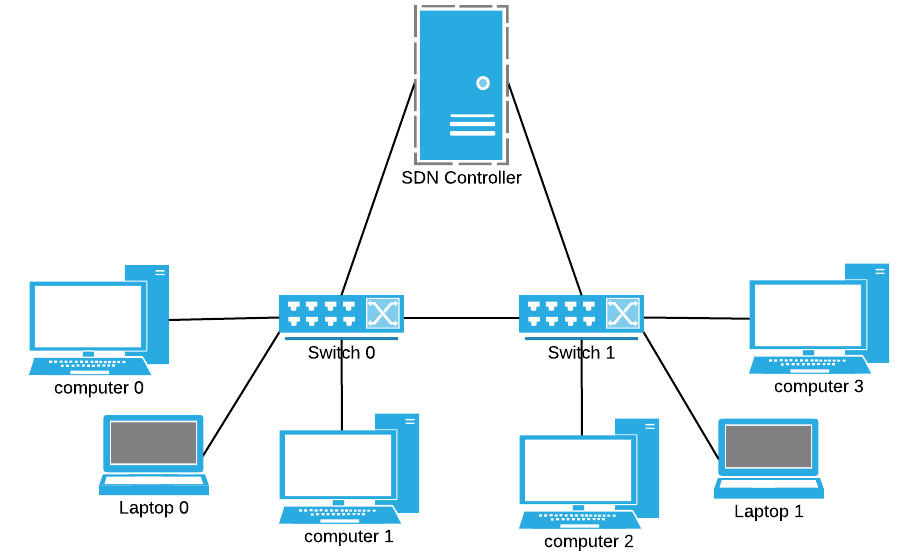
\includegraphics[scale=0.3]{img/simple-topology.png}
    \end{figure}

\end{frame}



%
% Detection log 
%
\begin{frame}[fragile]\frametitle{Detection}


\begin{figure}[h!]
\centering
\begin{lstlisting}[]
INFO:topology.graph:SwitchJoin id: 2
INFO:topology.graph:SwitchJoin id: 1
INFO:topology.graph:1, 2
DEBUG:openflow.discovery:Dropping LLDP packet 275
INFO:topology.graph:LinkEvent fired
INFO:host\_tracker:Learned 1 1 7e:e6:9b:89:39:2e got IP 10.0.0.1
INFO:topology.graph:HostJoin id: 7e:e6:9b:89:39:2e
INFO:host\_tracker:Learned 2 1 62:77:44:24:13:49 got IP 10.0.0.2
INFO:topology.graph:HostJoin id: 62:77:44:24:13:49
\end{lstlisting}
\caption{Entity Detection}
\label{fig:detection}
\end{figure}
\end{frame}



%
% Removing hosts
%
\begin{frame}\frametitle{Detecting departure of hosts}

    \begin{itemize}
        \item \emph{host\_tracker} periodically probes hosts using ARP requests
            for their addresses
        \item Requests are sent using Openflow to switch directly attached to
            the host
        \item HostLeave events are triggered after a configurable timeout 
        \item Associated edge is removed from the \emph{graph}
    \end{itemize}

\end{frame}



%
% Removing switch 
%
\begin{frame}\frametitle{Detecting the departure of switch}

    \begin{itemize}
        \item Switches connect to the controller by an Openflow control
            connection
        \item SwitchLeave event are triggered when the connection closes
        \item The switch vertex is removed; all hosts and edges 
              connected to it are also removed
    \end{itemize}

\end{frame}



%
% Online network traffic
%
\begin{frame}\frametitle{Online network traffic information}

    Edges are annoted with the observed traffic using Openflow counters
	\begin{figure}[h]
        \centering
        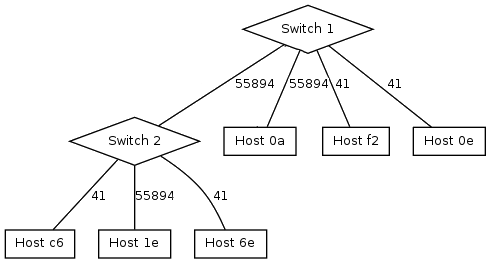
\includegraphics[scale=0.6]{img/iperf}
    \end{figure}

\end{frame}


%
% environment
%
\begin{frame}\frametitle{Experiments environment - Mininet}

    Contributions to Mininet:

    \begin{itemize}
        \item Methods to add/remove controllers, hosts, switches and links
        \item Extension of the class CLI
        \item Dynamic topology (enables usecases)
    \end{itemize}

\end{frame}



%
% Network representatation experiment
%
\begin{frame}\frametitle{Network representation}

    \begin{itemize}
        \item Experiment: build a network with 248 network entities
        \begin{itemize}    
            \item 8 switches
            \item Each switch with 30 directly connected to it
        \end{itemize}
    \end{itemize}

\end{frame}


%
% Network representation
%
\begin{frame}\frametitle{Network representation}

	\begin{figure}[h]
        \centering
        \hspace*{-1cm}
        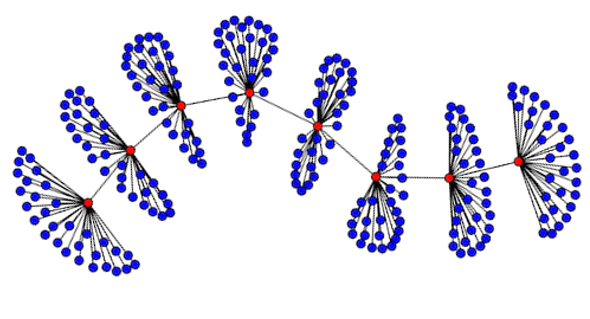
\includegraphics[scale=4.0]{img/full-graph}
    \end{figure}
\end{frame}


%
% Network representation
%
\begin{frame}\frametitle{Graph update times}
   
    

    \begin{table}
        \centering
        \scalebox{2.0}{%
        \begin{tabular}{l|ll}
            Entity  & Add & Remove \\
            \hline
            Host    & 1 & 30 \\
            Switch  & 0 & 0 \\
            Link    & 0 & 1  \\
        \end{tabular}}
    \caption{Update time of each action}
    \end{table}
\end{frame}


%
% API
%
\begin{frame}\frametitle{Application Programming Interface}

    \begin{itemize}
        \setlength{\itemsep}{10pt}
        \item \textbf{get\_vertex(vertex\_id)}; Returns a Vertex object
        \item \textbf{get\_adjacents(vertex)}; Returns a list of Vertexes objects
        \item \textbf{snapshot()}; Returns a dirt copy of the graph object
        \item \textbf{to\_dot()}; Returns the graph on DOT format
        \item \textbf{get\_mst()}; Returns the minimum spanning tree as a list
        \item \textbf{getters \& setters}; (vertexes and edges attributes)
    \end{itemize}

\end{frame}




%
% MST
%
\begin{frame}\frametitle{Example application: Minimum spanning tree}

    \begin{itemize}
        \item No need for distributed \emph{flood} algorithm 
        \item The implementation subscribes to join/leave events and recomputes
            the MST when required by events
        \item Load balancing may be used by observing links with lower traffic
        \item It is simple to implement solutions like Green MST (energy consuption)
    \end{itemize}

\end{frame}
